\section{RCD inside PADAR}\label{sec:rcd-pending-return}

\begin{definition}[RCD]
RCD names PADAR's duration coordinate when that coordinate is isolated for boundary accounting. For a returned-current channel
\[
\ADAR_e=(A_e,D_e,R^{\mathrm{asym}}_e),
\]
\(D_e(\partial F,\omega)\) is retained cut-return duration on the declared boundary/window. RCD is the local name for this duration coordinate together with its asymmetric reflection relation:
\[
\RCD_e = D_e\leftrightarrow R^{\mathrm{asym}}_e.
\]
\end{definition}

\paragraph{Windowed duration.}
Formulas use the PADAR duration coordinate:
\[
\min\!\left(D_e(\partial F,\omega),|\omega|_e\right).
\]
The minimum records the portion of the returned-current duration visible inside the declared window.

\begin{definition}[Pending duon pressure from a source]
For source field \(F_j\), receiver field \(F_i\), path \(\rho\), and declared boundary/window \((\partial F,\omega)\), define
\[
P^D_{i\leftarrow j,\rho}(\partial F,\omega)
=
\sum_{e:j\to i}
C_{3,e}\min\!\left(D_e(\partial F,\omega),|\omega|_e\right).
\]
\end{definition}

\paragraph{Self and cross cases.}
The diagonal \(i=j\) is self-field reflected return. The off-diagonal \(i\ne j\) is cross-field reflected return. Both use the same duration coordinate inside returned-current PADAR channels.

\paragraph{Poly duration/reflection coupling.}
A field with several shell or knot-return paths carries a family of duration/reflection couplings
\[
\left\{D_{e,\rho}(\partial F,\omega)\leftrightarrow R^{\mathrm{asym}}_{e,\rho}(\partial F,\omega)\right\}_{\rho}.
\]
These couplings belong inside PADAR because PADAR is poly-return field dynamics.

\begin{figure}[H]
\centering
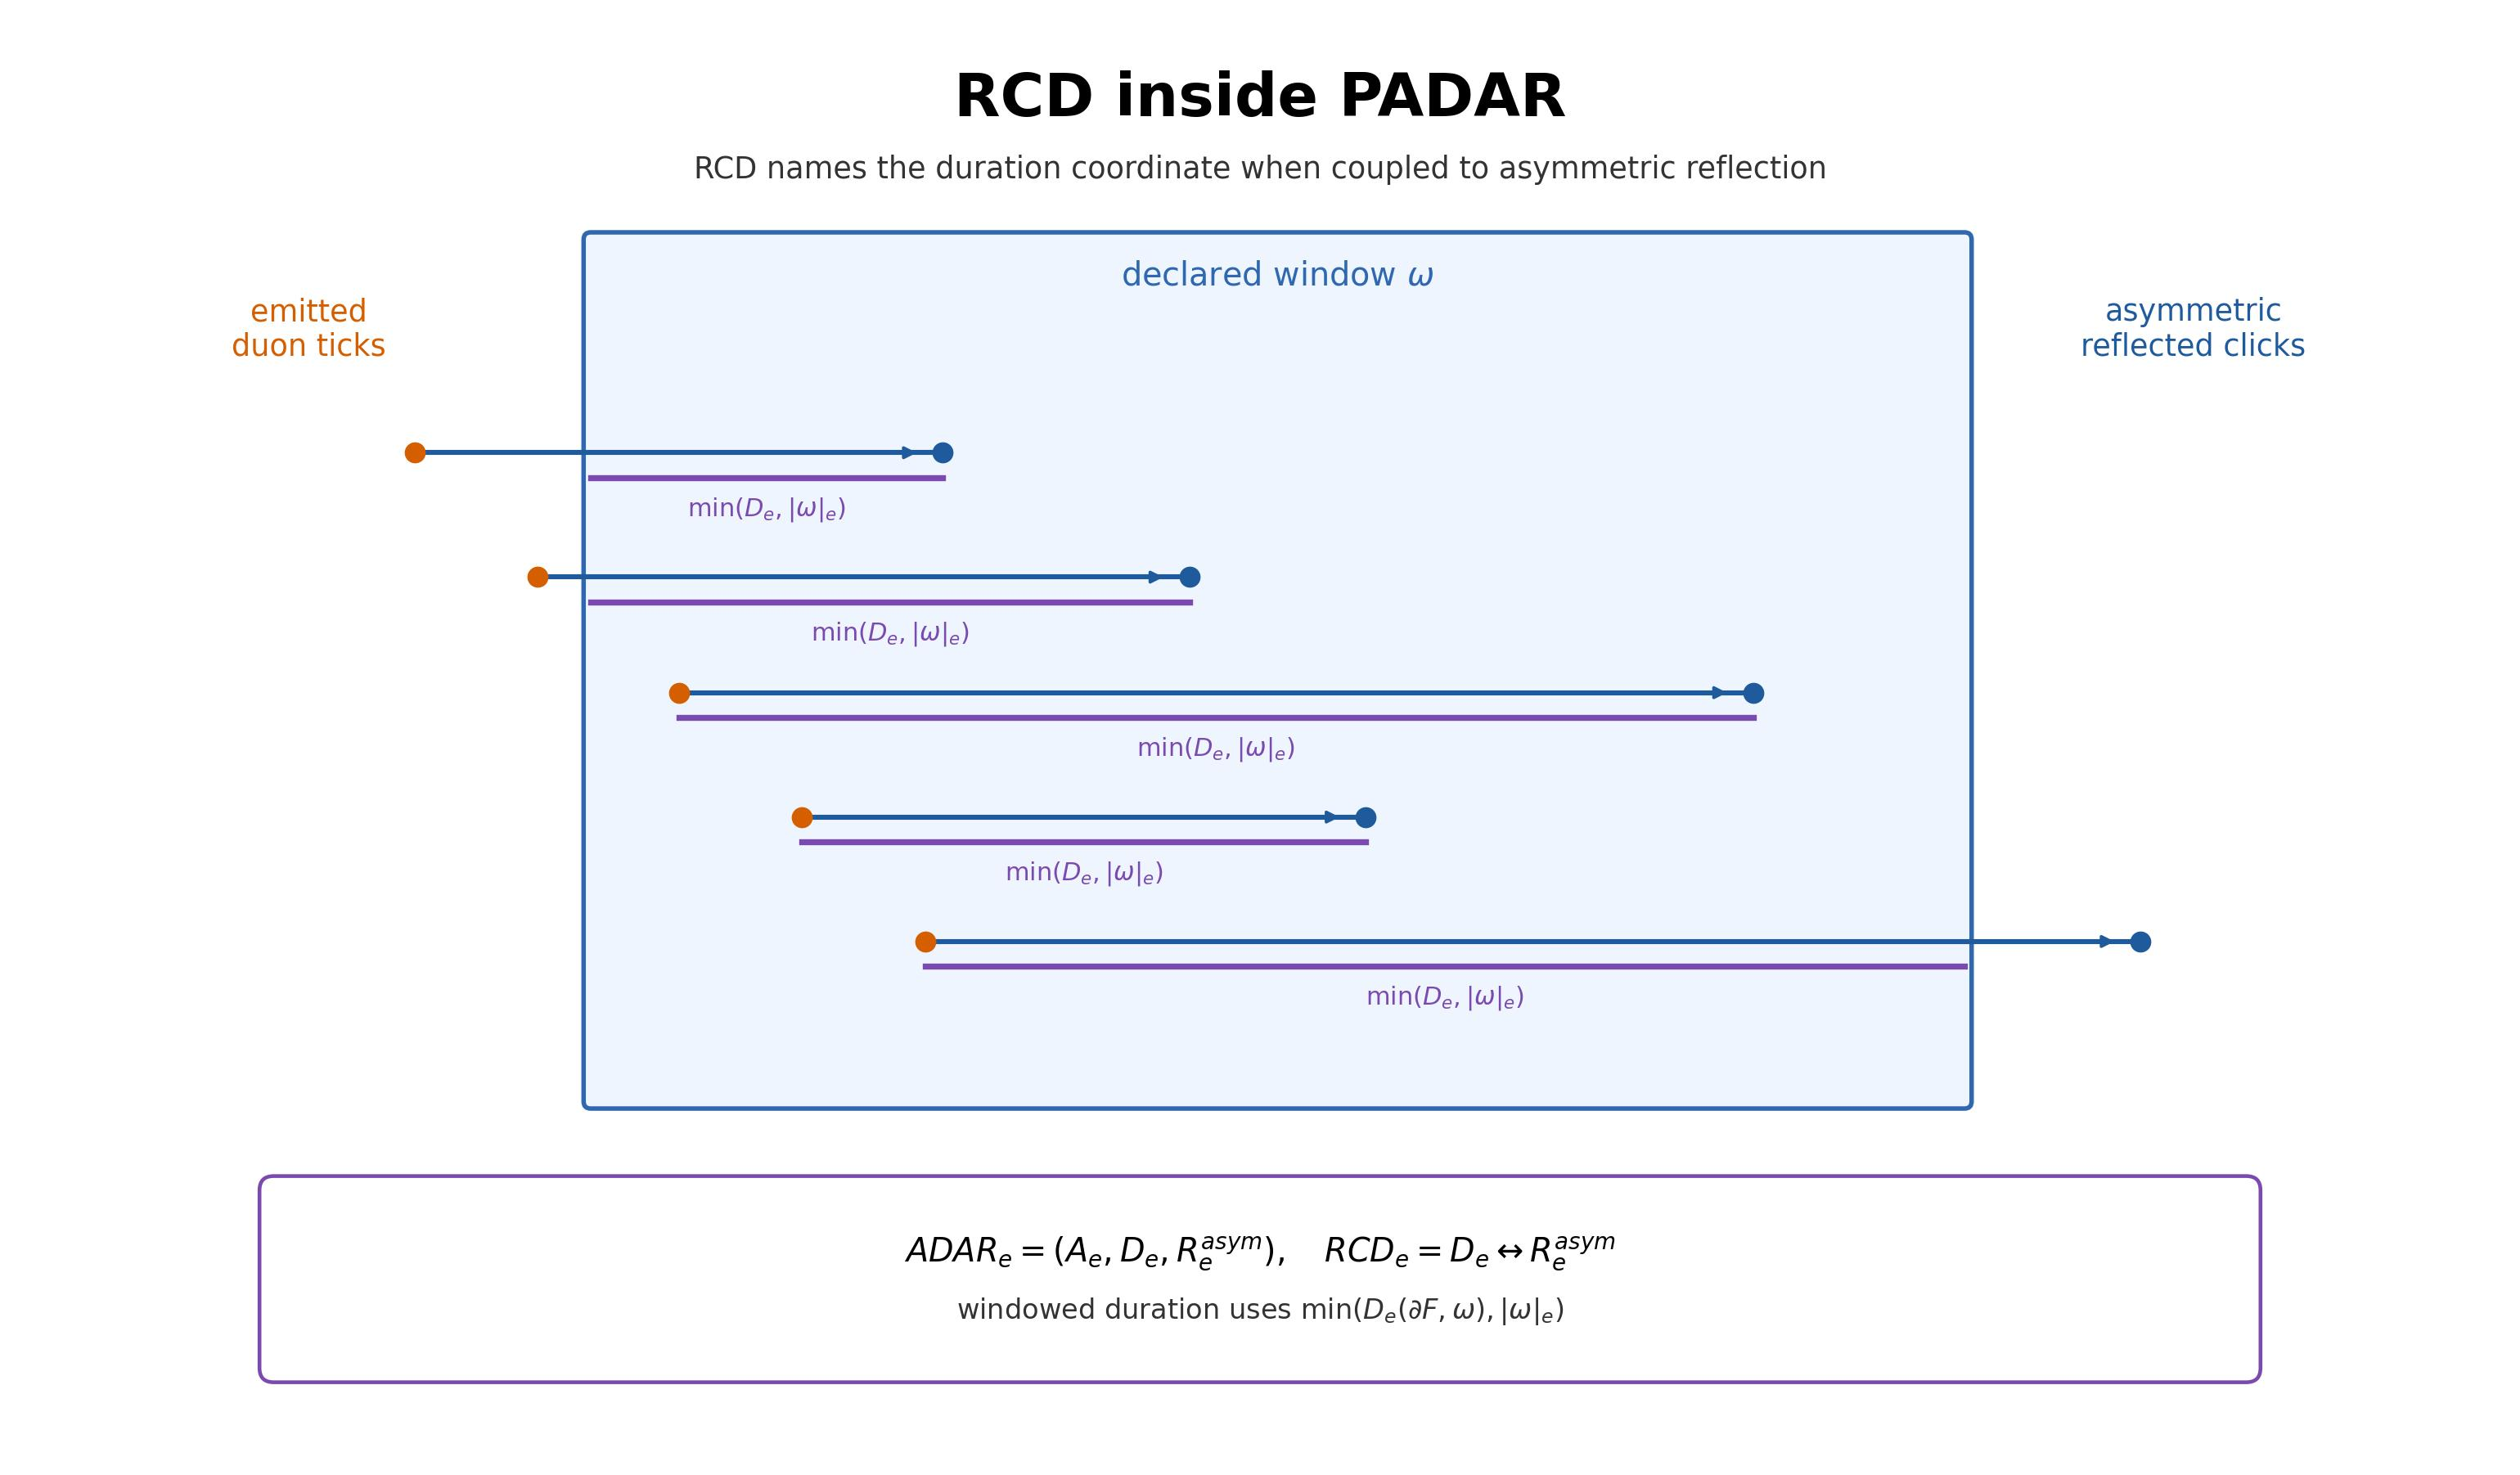
\includegraphics[width=0.98\linewidth]{figures_jpg/v39_16_rcd_reflection_duration_coupling.jpg}
\caption{RCD as windowed duration/reflection coupling. Outbound ticks remain coupled to reflected clicks; the visible bars show the pending-duration window inside the declared window.}
\label{fig:v39-rcd-pending-return}
\end{figure}
